% LTeX: language=it

\section{Goniometria}

Un angolo può essere misurato in gradi o radianti, infatti si ha $\alpha^{\circ}=\alpha[rad] \frac{180^{\circ}}{\pi}$.
Considerando una circonferenza goniometrica (raggio $r=1$), un angolo orientato $\alpha$, dal prolungamento del lato dell'angolo $\alpha$, otteniamo l'intersezione $B$, dove:

\begin{figure}[H]
    \centering
    % \begin{tikzpicture}
    %     \begin{axis}[
    %             unit vector ratio* = 1 1 1,
    %             clip=false,
    %             width=\textwidth,
    %             height=0.5*\textwidth,
    %             axis lines = middle,
    %             ymax=1.5,
    %             ymin=-1.5,
    %             xmax = 1.5,
    %             xmin = -1.5,
    %             xtick = {-1, 0, 1},
    %             ytick = {-1, 0, 1}
    %         ]
    %     \end{axis}
    %     % \draw (-1,0) node[left] {$(-1,0)$} -- (1,0) node[right] {$(1,0)$};
    %     % \draw (0,-1) node[below] {$(0,-1)$} -- (0,1) node[above] {$(0,1)$};
    %     \draw (center) coordinate (O) circle (1);
    %     \draw[red, very thick] (30:1cm) coordinate (B) -- (0,0-|B) coordinate(Bx) node[midway,left]{$\sin\alpha$};
    %     \draw [very thick,orange] (1,0) -- (intersection cs: first line={(O)--(B)},second line={(3,0)--(3,3)}) coordinate(B') node[midway,right]{$\tan\alpha$};
    %     \draw (O) -- (B');
    %     \draw[very thick,blue] (O) -- (Bx) node[midway,below]{$\cos\alpha$};
    % \end{tikzpicture}
    \begin{tikzpicture}[scale=2]
        \draw[step=.5cm,gray,very thin] (-1.4,-1.4) grid (1.4,1.4);
        \filldraw[fill=blue!20,draw=red] (0,0) -- (3mm,0mm)
        arc [start angle=0, end angle=30, radius=3mm] -- cycle;
        \node[red] at (15:2mm) {$\alpha$};
        \draw[->] (-1.5,0) -- (1.5,0) coordinate (x axis)node[right]{$x$};
        \draw[->] (0,-1.5) -- (0,1.5) coordinate (y axis)node[above]{$y$};
        \draw (0,0) circle [radius=1cm];
        \draw[very thick,orange]
        (30:1cm) -- node[left=1pt,fill=white] {$\sin \alpha$} (30:1cm |- x axis);
        \draw[very thick,blue]
        (30:1cm |- x axis) -- node[below=2pt,fill=white] {$\cos \alpha$} (0,0);
        \path [name path=upward line] (1,0) -- (1,1);
        \path [name path=sloped line] (0,0) -- (30:1.5cm);
        \draw [name intersections={of=upward line and sloped line, by=t}]
        [very thick,red] (1,0) -- node [right=1pt,fill=white]
        {$\displaystyle \tan \alpha$} (t);
        \draw (0,0) -- (t);
        \foreach \x/\xtext in {-1, -0.5/-\frac{1}{2}, 1}
        \draw (\x cm,1pt) -- (\x cm,-1pt) node[anchor=north,fill=white] {$\xtext$};
        \foreach \y/\ytext in {-1, -0.5/-\frac{1}{2}, 0.5/\frac{1}{2}, 1}
        \draw (1pt,\y cm) -- (-1pt,\y cm) node[anchor=east,fill=white] {$\ytext$};
    \end{tikzpicture}
\end{figure}

$y_B = \sin(\alpha) \qquad x_B = \cos(\alpha)$
$\frac{y_B}{x_B} = \tan(\alpha)$

Al variare dell'angolo $\alpha$, le funzioni vengono così rappresentate:

\begin{figure}[H]
    \centering
    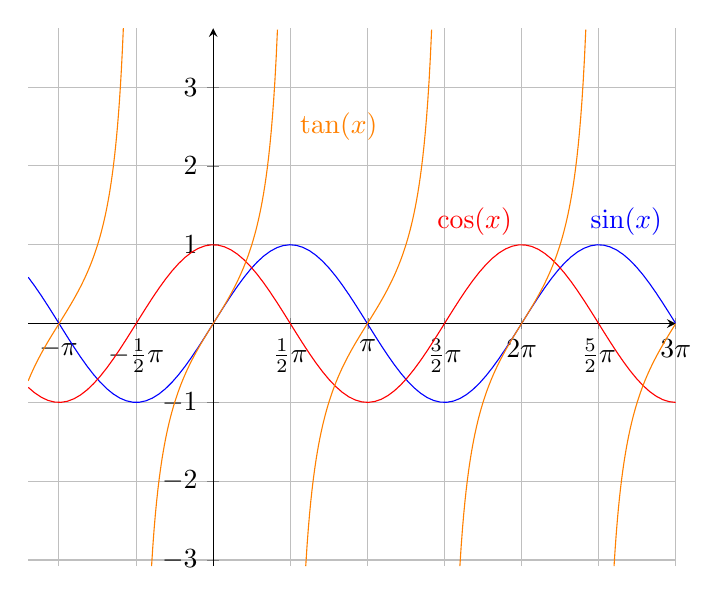
\begin{tikzpicture}
        \begin{axis}[enlargelimits=false,
                axis lines=middle,
                scale=1.2,
                xtick={-3.15159, -1.57080, 0,
                        1.57080,  3.15159, 4.71239,
                        6.28318,  7.85398, 9.42478 },
                xticklabels={$-\pi$, $-\frac{1}{2}\pi$, 0,
                        $\frac{1}{2}\pi$, $\pi$, $\frac{3}{2}\pi$,
                        $2\pi$, $\frac{5}{2}\pi$, $3\pi$ },
                ytick={-3,-2,-1,0,1,2,3},
                grid=major, % only a grid on the defined ticks
                samples=100 % number of points
            ]

            % sin
            \addplot[blue,no marks,domain=-1.2*pi:3*pi]{sin(deg(x))}; % deg to convert radians
            \node[right=10pt,above] at (axis cs:5*pi/2,1){\color{blue}$\sin(x)$};

            % cos
            \addplot[red,no marks,domain=-1.2*pi:3*pi] {cos(deg(x))};
            \node[above left] at (axis cs:2*pi,1){\color{red}$\cos(x)$};

            % tan, multiple parts because of singularities
            \addplot[orange,no marks,domain=-1.2*pi:-0.583*pi, ]{tan(deg(x))};
            \addplot[orange,no marks,domain=-0.4*pi:5*pi/12,   ]{tan(deg(x))};
            \addplot[orange,no marks,domain=27*pi/45:17*pi/12, ]{tan(deg(x))};
            \addplot[orange,no marks,domain=1.6*pi:29*pi/12,   ]{tan(deg(x))};
            \addplot[orange,no marks,domain=2.6*pi:36*pi/12,   ]{tan(deg(x))};
            \node[right] at (axis cs:pi/2,2.5){\color{orange}$\tan(x)$};

        \end{axis}
    \end{tikzpicture}
\end{figure}

Tutte queste funzioni sono periodiche, per cui $f(x) = f(x+T)$, dove $T$ è il periodo della funzione.

Angoli noti:

\begin{table}[H]
    \centering
    \begin{tabular}{|l|l|l|l|}
        \hline
        Angolo $^{\circ}$ & $\sin(\alpha)$        & $\cos(\alpha)$        & $\tan(\alpha)$       \\ \hline
        0                 & $0$                   & $1$                   & $0$                  \\ \hline
        30                & $\frac{1}{2}$         & $\frac{\sqrt{3}}{2}$  & $\frac{1}{\sqrt{3}}$ \\ \hline
        45                & $\frac{\sqrt{2}}{2} $ & $\frac{\sqrt{2}}{2} $ & $1$                  \\ \hline
        60                & $\frac{\sqrt{3}}{2}$  & $\frac{1}{2}$         & $\sqrt{3}$           \\ \hline
        90                & $1$                   & $0$                   & $\infty$             \\ \hline
    \end{tabular}
\end{table}

Esistono poi le funzioni inverse, che permettono di trovare l'angolo $\alpha$ a partire da un dato valore della funzione (es. $\sin(30^{\circ}) = \frac{1}{2} \rightarrow 30^{\circ} = \arcsin(\frac{1}{2})$).

\begin{figure}[H]
    \centering
    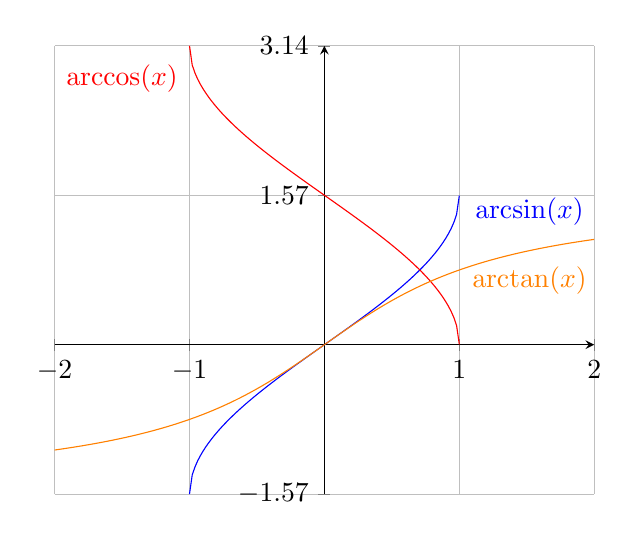
\begin{tikzpicture}
        \begin{axis}[enlargelimits=false,
                axis lines=middle,
                xtick={-2,-1,0,1,2},
                ytick={-1.570780, 1.570780, 3.14159},
                % yticklabels={$-\frac{1}{2}\pi$,$\frac{1}{2}\pi$,$\pi$},
                grid=major,
                samples=100
            ]

            % arcsin
            \addplot[domain=-1:1,no marks,blue] {rad(asin(x))};
            \node at (axis cs:1.52,1.4){\color{blue}$\arcsin(x)$};

            % arccos
            \addplot[domain=-1:1,no marks,red] {rad(acos(x))};
            \node at (axis cs:-1.5,2.8){\color{red}$\arccos(x)$};

            % arctan
            \addplot[domain=-2:2,no marks,orange] {rad(atan(x))};
            \node at (axis cs:1.52,.67){\color{orange}$\arctan(x)$};

        \end{axis}
    \end{tikzpicture}
\end{figure}

Il periodo $T$ di una funzione si ricava come: $f(x)=\sin(\omega x) \rightarrow T=\frac{2\pi}{\omega}$

Relazioni fondamentali della goniometria: $\sin(\alpha)^2 + \cos(\alpha)^2 = 0$ e $\frac{\sin(\alpha)}{\cos(\alpha)} = \tan(\\alpha)$

\subsection{Funzioni goniometriche}

\subsubsection*{Addizione}

\begin{align}
    \sin(\alpha+\beta) & = \sin(\alpha)\cos(\beta)+\cos(\alpha)\sin(\beta)
    \label{eq:goniometria_formule_di_addizione_seno}                                  \\
    \cos(\alpha+\beta) & = \cos(\alpha)\cos(\beta)-\sin(\alpha)\sin(\beta)
    \label{eq:goniometria_formule_di_addizione_coseno}                                \\
    \tan(\alpha+\beta) & = \frac{\tan(\alpha)+\tan(\beta)}{1-\tan(\alpha)\tan(\beta)}
    \label{eq:goniometria_formule_di_addizione_tangente}
\end{align}

\subsubsection*{Sottrazione}
\begin{align}
    \sin(\alpha-\beta) & = \sin(\alpha)\cos(\beta)-\cos(\alpha)\sin(\beta)
    \label{eq:goniometria_formule_di_sottrazione_seno}                                \\
    \cos(\alpha-\beta) & = \cos(\alpha)\cos(\beta)+\sin(\alpha)\sin(\beta)
    \label{eq:goniometria_formule_di_sottrazione_coseno}                              \\
    \tan(\alpha-\beta) & = \frac{\tan(\alpha)-\tan(\beta)}{1+\tan(\alpha)\tan(\beta)}
    \label{eq:goniometria_formule_di_sottrazione_tangente}                            \\
\end{align}

\subsubsection*{Duplicazione}
\begin{align}
    \sin(2\alpha) & = 2\sin(\alpha)\cos(\alpha)
    \label{eq:goniometria_formule_di_duplicazione_seno}                      \\
    \cos(2\alpha) & = \cos^2(\alpha)-\sin^2(\alpha)
    \label{eq:goniometria_formule_di_duplicazione_coseno}                    \\
    \tan(2\alpha) & = 2\tan(\alpha)\frac{1-\tan^2(\alpha)}{1+\tan^2(\alpha)}
    \label{eq:goniometria_formule_di_duplicazione_tangente}
\end{align}

\subsubsection*{Bisezione}
\begin{align}
    \sin(\frac{\alpha}{2}) & = \pm\sqrt{\frac{1-\cos(\alpha)}{2}}
    \label{eq:goniometria_formule_di_bisezione_seno}                                                                                                          \\
    \cos(\frac{\alpha}{2}) & = \pm\sqrt{\frac{1+\cos(\alpha)}{2}}
    \label{eq:goniometria_formule_di_bisezione_coseno}                                                                                                        \\
    \tan(\frac{\alpha}{2}) & = \pm\frac{\sqrt{1-\cos(\alpha)}}{\sqrt{1+\cos(\alpha)}}=\frac{\sin(\alpha)}{1+\cos(\alpha)}=\frac{1-\cos(\alpha)}{\sin(\alpha)}
    \label{eq:goniometria_formule_di_bisezione_tangente}
\end{align}

% \subsubsection*{Prodotto}
% \begin{align}
%     \sin(\alpha)\sin(\beta) & = \frac{1}{2}[\cos(\alpha-\beta)-\cos(\alpha+\beta)]
%     \label{eq:goniometria_formule_di_prodotto_seno}                                \\
%     \cos(\alpha)\cos(\beta) & = \frac{1}{2}[\cos(\alpha-\beta)+\cos(\alpha+\beta)]
%     \label{eq:goniometria_formule_di_prodotto_coseno}                              \\
%     \sin(\alpha)\cos(\beta) & = \frac{1}{2}[\sin(\alpha-\beta)+\sin(\alpha+\beta)]
%     \label{eq:goniometria_formule_di_prodotto_tangente}
% \end{align}

\subsubsection*{Parametriche}
\begin{align}
    \sin(\alpha) & = \frac{2\tan(\frac{\alpha}{2})}{1+\tan^2(\frac{\alpha}{2})}
    \label{eq:goniometria_formule_parametriche_seno}                               \\
    \cos(\alpha) & = \frac{1-\tan^2(\frac{\alpha}{2})}{1+\tan^2(\frac{\alpha}{2})}
    \label{eq:goniometria_formule_parametriche_coseno}                             \\
    \tan(\alpha) & = \frac{2\tan(\frac{\alpha}{2})}{1-\tan^2(\frac{\alpha}{2})}
    \label{eq:goniometria_formule_parametriche_tangente}
\end{align}

\subsubsection*{Esistono anche}
\begin{align}
    \sin^2(\alpha) & = \frac{1-\cos(2\alpha)}{2}
    \label{eq:goniometria_formule_seno_al_quadrato}   \\
    \cos^2(\alpha) & = \frac{1+\cos(2\alpha)}{2}
    \label{eq:goniometria_formule_coseno_al_quadrato} \\
\end{align}

Ogni formula contenente la tangente ha le sue condizioni di esistenza.
In generale essendo $\tan(\alpha)=\frac{\sin(\alpha)}{\cos(\alpha)}$ si ha che $\tan(\alpha)$ esiste se $\cos(\alpha)\neq0$, ovvero se $\alpha\neq K\pi$ con $K \in Z$.


\subsection{Equazioni goniometriche}

Esistono diversi tipologie di equazioni goniometriche.

\subsubsection{Equazioni elementari}

Sfruttano il principio degli angoli associati:

\begin{equation*}
    \sin(\alpha)= \rightarrow
    \begin{cases}
        \alpha=\arcsin(\frac{1}{2}) \\
        \alpha=(\pi-\arcsin(\frac{1}{2}))
    \end{cases}
\end{equation*}

\subsubsection{Equazioni di 1° grado}

Qui distinguiamo due casi di omogenea (se tutti i termini sono dello stesso grado) e non omogenea.

\paragraph{Omogenea, $c = 0$}

Data l'equazione $A\sin(\alpha) + B\cos(\alpha) = 0$, la riconduco a una forma elementare dividendo i termini per $\cos(\alpha)$ e ottenere così:

\begin{equation*}
    A\tan(\alpha)+B = 0 \rightarrow \tan(\alpha) = -\frac{A}{B}
\end{equation*}

\paragraph{Non omogenea, $c \neq 0$}

Data l'equazione $A\sin(\alpha) + B\cos(\alpha) + C= 0$, esistono tre modi per risolverla:

\begin{itemize}
    \item Parametrico: pongo $sin(\alpha) = \frac{2T}{1+T^2}$ e $cos(\alpha) = \frac{1-T^2}{1+T^2}$, con $T = \tan(\frac{\alpha}{2})$.
    \item Grafico: pongo $Y =\sin(\alpha)$ e $X = \cos(\alpha)$, e metto a sistema
          \[
              \begin{cases}
                  AY + BX + C = 0 \\
                  X^2 + Y^2 = 1
              \end{cases}
          \]
          Le intersezioni trovate corrispondono alle soluzioni.
    \item Angolo aggiunto: considero l'equazione $A\sin(\alpha) + B\cos(\alpha) + C = 0$  come se fosse la formula di addizione (\ref{eq:goniometria_formule_di_addizione_seno}) di $\sin(\alpha + \beta) = \sin(\alpha)\cos(\beta)+\cos(\alpha)\sin(\beta) = - C$, dove $\cos(\beta) = A$ e $\sin(\beta) = B$ \\
          Calcolo dunque il raggio della circonferenza come $r = \sqrt{A^2 + B^2}$ e divido il tutto per $r$. \\
          Trovo dunque $\alpha$ avendo il valore di $\cos(\alpha)$ e $\sin(\alpha)$, e riduco a equazione elementare $\sin(\alpha + \beta) = -\frac{C}{2} \rightarrow \alpha = \arcsin(-\frac{C}{2}) - \beta$
\end{itemize}

Esempio angolo aggiunto:

\begin{gather}
    \cos(\alpha) - \sqrt{3}\sin(\alpha) = 1 \rightarrow r = \sqrt{1^2 + (\sqrt{3})^2} = 2 \\
    \begin{cases}
        \cos(\beta) = \frac{1}{2} \\
        \sin(\beta) = -\frac{\sqrt{3}}{2}
    \end{cases}
    \rightarrow \beta = \frac{5\pi}{6} \\
    \sin(\alpha + \frac{5\pi}{6}) = \frac{1}{2} \rightarrow \begin{cases}
        \alpha + \frac{5\pi}{6} = \frac{\pi}{6} + 2k\pi \rightarrow \alpha = -\frac{2\pi}{3} + 2k\pi \\
        \alpha + \frac{5\pi}{6} = \frac{5\pi}{6} + 2k\pi \rightarrow \alpha = 0 + 2k\pi
    \end{cases}
\end{gather}

\subsubsection{Equazioni di 2° grado}

Definite nella forma $A\sin^2(\alpha) + B\cos(\alpha)\sin(\alpha) + C\cos^2(\alpha) + D = 0$, si risolvono in maniera differente a seconda del valore di $D$.

\paragraph{Caso 1, $D = 0$}

Si raccoglie $\sin(\alpha)$ o $\cos(\alpha)$ se $A = 0$ o $C = 0$ rispettivamente, e si risolve come un'equazione di 1° grado.
Altrimenti si divide per $\cos^2(\alpha)$ e otteniamo $A\tan^2(\alpha) + B\tan(\alpha) + C = 0$, e si risolve come un'equazione di 2° grado ponendo $x = \tan(\alpha)$.

\paragraph{Caso 2, $D \neq 0$}

Si riscrive $D$ come $D = D\sin^2(\alpha) + D\cos^2(\alpha)$, e si arriva quindi ad avere $A\sin^2(\alpha) + B\cos(\alpha)\sin(\alpha) + C\cos^2(\alpha) + D\sin^2(\alpha) + D\cos^2(\alpha) = 0$.
Proseguo dividendo per $cos^2(\alpha)$ e riportandomi dunque al caso sopra descritto.


\subsection{Disequazioni goniometriche}

Per risolvere una disequazione goniometrica, si ricava da prima la soluzione dell'equazione associata come descritto sopra, e si utilizza poi la circonferenza come grafico per determinare il segno.

\begin{gather}
    (2\sin(\alpha) + \sqrt{2})(2\cos(\alpha) - 1) > 0 \\
    \begin{cases}
        2\sin(\alpha) + \sqrt{2} > 0 \\
        2\cos(\alpha) - 1 > 0
    \end{cases}
    =
    \begin{cases}
        \sin(\alpha) > -\frac{1}{\sqrt{2}} \\
        \cos(\alpha) > \frac{1}{2}
    \end{cases}
    \rightarrow
    \begin{cases}
        -\frac{\pi}{4} < \alpha < \frac{5\pi}{4} \\
        -\frac{\pi}{3} < \alpha < \frac{\pi}{3}
    \end{cases}
\end{gather}

% TODO: graph

Dal grafico si vede che la soluzione è $-\frac{\pi}{4} < \alpha < \frac{\pi}{3} \vee \frac{5\pi}{4} < \alpha < \frac{5\pi}{4}$.

